\chapter{Fixed media}

\section{Framework and historical context}\label{framework-and-historical-context}

The first musical works recorded on media were created in the 1950s in the Radio France studios in Paris by composers belonging to the Groupe de recherches musicales (GRM) by Pierre Schaeffer.

Composers such as Pierre Henry, François Bayle, Bernard Parmegiani, Christian Zanési and Daniel Teruggi have collaborated with this institute.

These composers, more or less, referred to Schaeffer’s sound theories about "musique concrete" later outlined in his book  \textit{Traité des Objects Musicaux}.

The design of the studio followed strict Schaefferian theory and was completely centered around tape manipulation, recording and editing.

Two main electroacoustic instruments:

\begin{itemize}
\tightlist
\item phonogène \(\rightarrow\) a multi-headed tape instrument in three versions:
    \begin{itemize}
    \tightlist
    \item Chromatic phonogène. Tape loop at varied speeds. It produced short bursts of tape sounds at varying pitches defined by a small one-octave keyboard.
    \item Sliding phonogène. It produced continuous tone by varying the tape speed via a control rod.
    \item Phonogène Universal. It allowed time stretching without transposing the pitches and vice versa obtained through a rotating magnetic head.
    \end{itemize}
\item morphophone \(\rightarrow\)  a type of tape loop-delay mechanism. The sound was picked up at varying points on the tape by ten magnetic heads (one recording, one erasing and ten playback heads) then passed through ten bandpass fileters (one for each head).
\end{itemize}

Theories of musique concrète are based on the concept of a \textit{sound object}.

\section{Elements and strategies}\label{elements-and-strategies}

In this section we outline some concepts underlying any compositional process.

They are valid in subsequent chapters where we will explore the
specifics.

They are some of the main tools of composing electronic music.

\subsection{Sound objects}\label{sound-objects}

\begin{center}
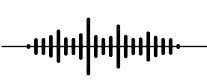
\includegraphics[scale=0.4]{../img/sound.png}
\end{center}

Let's explore the concepts of sound object.

Pierre Schaeffer in his \textit{Traité des objets musicaux} (1966) wrote:

\textit{Let's assume a single microphone:}

\begin{itemize}
\tightlist
\item \textit{it is the point of convergence of all the soundwaves arriving from the sound points in the surrounding space.}
\item \textit{all the sound points in the initial space will be condensed into the microphone's membrane.}
\item \textit{the initial surrounding space is replaced by a sound point.}
\item \textit{if we play back it, it generates a new sound distribution in a new surrounding space.}
\item \textit{the diffusion medium (loudspeaker) is neutral favoring an acousmatic sound perception.}
\item \textit{we can consider this sound point as a word, a representation, not a recording of reality.}
\item \textit{we can call this representation a \textit{sound object}.}
\end{itemize}

A sound object is any sound phenomenon perceived:

\begin{itemize}
\tightlist
\item as a coherent whole.
\item heard in an acousmatic situation, regardless of its origin and meaning.
\end{itemize}

P.Henry - \href{https://github.com/musicaecodice/EMC/blob/main/3_fixed/suoni/henry.mp3}{Futuriste} for tape (1975)

\subsection{Objects, structure and form }\label{objects-structure-and-form}

\begin{center}
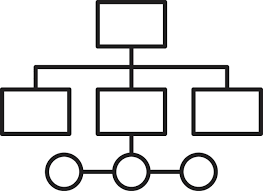
\includegraphics[scale=0.3]{../img/struc.png}
\end{center}

Schaeffer argues also that the object/structure pair is at the basis of our perceptual activity.

What is a structure?

A structure is a model the skeleton of a form.

What is a form?

General concept exposed by A.Lalande (Vocabulaire technique et critique de la philosophie):

\textit{Forms are sets, which constitute autonomous units, manifest an internal solidarity, and have their own laws.}

The nature of each element depends on the structure of the whole and the laws that govern it.

Neither psychologically nor physiologically does the element (object) pre-exist the whole.

The concept of form is therefore more complex than that of structure

Schaeffer illustrates this concept with two examples from western musical tradition:

\begin{itemize}
\tightlist
\item a melody cannot be reduced to the sequence of notes that compose it.
  \begin{itemize}
  \tightlist
  \item if when we listen to a melody we focus our attention on a single note, the perception of the melody vanishes.
  \item if we focus our attention on the entire melody (melodic profile) the perception of the individual notes vanishes.
  \end{itemize}
\item if the melody is in G major and we play an F natural we perceive a discordant note.

  \begin{itemize}
  \tightlist
  \item the musical scale is a structure that influences the encoding and decoding of the notes.
  \end{itemize}
\end{itemize}

Let us remember the continuous reference of the signs discussed in the paragraph about musical meaning.

Structure provides the relevant features that enable members of a musical tradition to encode and decode sounds.

In music, these structures are usually organized according to coherent variations of characterizing models (major, minor, etc.).

Schaeffer then aims to define a new sound vocabulary based on the intrinsic sound characteristics (morphosyntax) of sound objects.

Sound objects become musical objects.

\subsection{Musical objects}\label{musical-objects}

\begin{center}
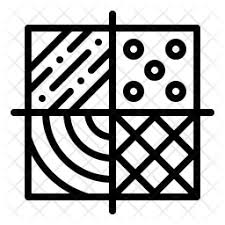
\includegraphics[scale=0.2]{../img/texture1.png}
\end{center}

When we start to write a sound or musical work on a fixed media we should define few procedures:

\begin{enumerate}
\tightlist
\item choose and/or define the sound material (recorded or synthetic) to be used in the piece (sound objects).

  This choice should be made by:

  \begin{itemize}
  \tightlist
  \item recorded sound objects \(\rightarrow\) analysis of their morphological characteristics (perception).
  \item synthesized sound objects \(\rightarrow\) definition of their morphological characteristics (idea of a sound).
  \end{itemize}

  In both cases (analysis or definition) we can employ some simple strategies derived from the much more complex theories of composers and musicologists such as P.Schaeffer, M.Chion, D.Smalley and others.

  We should think about:

  \begin{itemize}
  \tightlist
  \item mass \(\rightarrow\) (spectral) quality that describes its perceived consistency, density, or \textit{weight}.
    \begin{itemize}
    \tightlist
    \item pure sound (sinusoid).
    \item tonic sound - defined pitch harmonic spectra (instrument).
    \item tonic group (chord or melodic pattern whitin a range).
    \item mixed sound (ambiguos).
    \item node (tremolo or ribattuto).
    \item nodal group (texture of inharmonic sounds).
    \item noise (white, pink, etc.).
    \end{itemize}
  \item
    matter \(\rightarrow\) grain - texture - object surface.

    \begin{itemize}
    \item smooth (static).
      \begin{center}  
      
\includegraphics[scale=0.1]{../img/linea.png}
      \end{center}
    \item harmonica (trembling).
      \begin{center}
      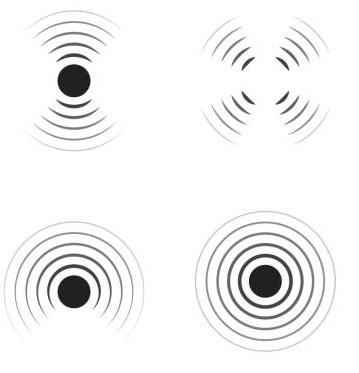
\includegraphics[scale=0.45]{../img/tremore.png}
      \end{center}
    \item compact harmonica (fluctuating).
      \begin{center}
      
\includegraphics[scale=0.1]{../img/scricchiolio.png}
      \end{center}
    \item compact (rustling).
      \begin{center}
      
\includegraphics[scale=0.1]{../img/fruscio.png}
      \end{center}
    \item compact discontinuous (rhombus).
      \begin{center}
      
\includegraphics[scale=0.2]{../img/rombo.png}
      \end{center}
    \item discontinuous (crackling).
      \begin{center}
      
\includegraphics[scale=0.22]{../img/crepitio.png}
      \end{center}
    \item discontinuous harmonic (squeak).
      \begin{center}
      
\includegraphics[scale=0.22]{../img/cigolio.png}
      \end{center}
    \item rhytmic (measured pattern).
      \begin{center}
      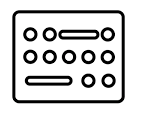
\includegraphics[scale=0.3]{../img/morse.png}
      \end{center}
    \end{itemize}
  \item dynamic.

    \begin{itemize}
    \tightlist
    \item global (dynamic profile) - if a sound object is fortissimo or piano or\ldots{}
    \item
      internal (grain envelopes) - dynamic evolution or contrast in internal parts.
    \end{itemize}
  \end{itemize}
  
  \begin{center}
  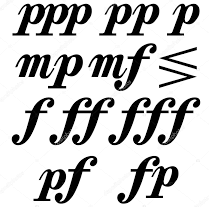
\includegraphics[scale=0.33]{../img/dyno.png}
  \end{center}

  Each of these parameters may or may not evolve over the course of the sound object in different ways:

  \begin{itemize}
  \item static (-) \(\rightarrow\) no evolution or small small fluctuations (tremolo, vibrato, beting, etc.).
    \begin{center}
    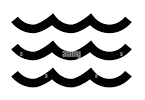
\includegraphics[scale=0.2]{../img/static.png}
    \end{center}
  \item opening (\textless) \(\rightarrow\) up glissando, crescendo, increase in density, etc.
    \begin{center}
    
\includegraphics[scale=0.1]{../img/open.png}
    \end{center}
  \item closing (\textgreater) \(\rightarrow\) down glissando, diminuendo, decrease in density, etc.
    \begin{center}
    
\includegraphics[scale=0.15]{../img/close.png}
    \end{center}
  \item alternated (\textless\textgreater) \(\rightarrow\) open and close like a pendoluum.
    \begin{center}
    
\includegraphics[scale=0.22]{../img/alternate.png}
    \end{center}
  \item variated \(\rightarrow\) variation in pattern (rhythmic or melodic or spactral, etc.).
    \begin{center}
    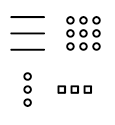
\includegraphics[scale=0.35]{../img/varia.png}
    \end{center}
  \item random \(\rightarrow\) non evolutive.
    \begin{center}
    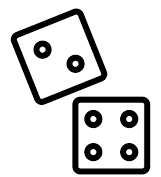
\includegraphics[scale=0.2]{../img/random.png}
    \end{center}
  \end{itemize}

  All these evolution can be fast or slow.
  
\item build a sound vocabulary (a sound palette) that includes one or more sets of sounds elaborated from those chosen in the previous point.

  The criteria adopted in generating this sound palette can be varied, including:

  \begin{itemize}
  \tightlist
  \item a set of coherent sound objects with morphological similarity to the original.
  \item a set of sound objects with gradual differentiation (direction, interpolation, etc.).
  \item a set of incoherent sound objects where the sound processing distort the original morphology.
  \end{itemize}

  The sound objects included in these sets become \textit{musical objects}  because they have acquired a semantic function within a system (such as the division of the octave into intervals of a scale in Western music theory).

\item order (compose) these sounds over time into different types of sound textures and paths, designing a musical form.

  The criteria we can adopt in doing so can include among others:

  \begin{itemize}
  \tightlist
  \item staticity - evolution - variation.
  \item continuity - discontinuity.
  \item contrast - uniformity.
  \item etc.
  \end{itemize}
\end{enumerate}

In this way we can construct and formalize an abstract thought.

Let's try to recognize musical objects, their characteristics and how they evolve over time in these extracts from B.Parmegiani works (\href{http://www.musicaecodice.it/gitmedia/emc/3_media/parme1.mp4}{extract1}, \href{http://www.musicaecodice.it/gitmedia/emc/3_media/parme2.mp3}{extract2}, \href{http://www.musicaecodice.it/gitmedia/emc/3_media/parme3.mp3}{extract3}).

\subsection{Time courses and musical forms}\label{time-courses-and-musical-forms}

Some further thoughts regarding time courses and musical forms.

In the figurative arts (architecture, painting, sculpture) forms exist in the dimension of space.

\begin{center}

\includegraphics[scale=0.4]{../img/scultura.png}
\end{center}

Musical forms are created over time.

\begin{center}

\includegraphics[scale=0.2]{../img/metronomo.png}
\end{center}

We cannot think of time in forms but only as events with different temporal courses.

\begin{center}
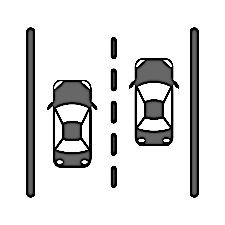
\includegraphics[scale=0.3]{../img/corsie.png}
\end{center}

A musical form can be defined as a thought that thinks about the course of events.

\begin{center}
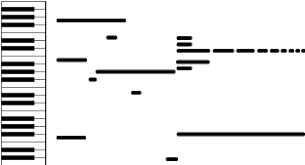
\includegraphics[scale=0.7]{../img/pianoroll.png}
\end{center}

In the temporal domain (and therefore in the musical domain) there are two main formal typologies:

\begin{itemize}
\tightlist
\item teleo-logical.
\item circular.
\end{itemize}

\textbf{Teleo-logical time}\label{teleo-logical-time}

This time-course is goal-oriented and plays a dominant role in Western music.

The mode of a \href{http://www.musicaecodice.it/gitmedia/emc/3_media/finalis.mp3}{medieval melody} is determined by the finalis which is the last event of the course.

In tonal harmony a dissonance tends toward \href{http://www.musicaecodice.it/gitmedia/emc/3_media/risolvi.mp3}{resolution} just as a cadence moves toward the closing tonic.

Over a longer time an opera or the movements of a symphony gravitate towards the Finale (micro and macro structure).

Tonality based on \href{http://www.musicaecodice.it/gitmedia/emc/3_media/aggregati.mp3}{harmonic functions} has a teleo-logical nature as the sound aggregates are constantly moving towards reference points.

A point-to-point movement.

Only at the end when we reach the final cadence \href{http://www.musicaecodice.it/gitmedia/emc/3_media/forma1.m4v}{the process of the whole} being formed into a figure temporally accomplished.

\textbf{Circular time}\label{circular-time}

Movement returns incessantly to itself; it has no goal, no beginning, and no end.

In Western music, it appears:

\begin{itemize}
\tightlist
\item in the dissolution of functional harmony (early 1900) - \href{http://www.musicaecodice.it/gitmedia/emc/3_media/mal.mp3}{exemple}.
\item in phenomena of the serial or stochastic pointillistic form (mid 1900) - \href{http://www.musicaecodice.it/gitmedia/emc/3_media/web.mp3}{exemple}.
\item in phenomena of the anvantgarde and experimental music (after 1950) - \href{http://www.musicaecodice.it/gitmedia/emc/3_media/mont.mp3}{exemple}.
\end{itemize}

Music is de-teleologized and de-temporalized, eliminating any defined profile.

Thought that considers the process frees itself from the chains that bind it to hierarchies and the need to strive toward a goal.

A typical position of Eastern philosophies, thought seeks to free itself from all limitations to achieve the unity of being.

The concept of time in music has always historically stemmed from a general reflection.

For this reason, today we can choose which temporal typology to adopt to best construct the desired musical form.

\subsection{The poietic dimension: determinism}\label{the-poietic-dimension-determinism}

In the previous chapter we saw that the musicologist J.J.Nattiez defines the poietic dimension as the set of strategies activated by the author that lead to the creation of the work (something that did not exist before).

As for the simple organization of sounds over time, stripped of all other components that contribute to their creation, the processes we can employ in design and implementation are essentially two types:

\begin{itemize}
\tightlist
\item deterministic procedures.
\item stochastic procedures.
\end{itemize}

We will deal with the first type in this paragraph while the second in the next chapter on computer music.

In philosophical and scientific language, determinism is a conception according to which the events of metaphysical, physical, or moral reality are necessarily and invariably connected to each other.

If we make this choice when composing a piece, we face two options:

\begin{itemize}
\tightlist
\item use our \textit{libero arbitrio} and choose all the parameters at our own discretion (not randomly, but according to a specific intention).
\item follow or create systems of rules to generate or transform some or all of the parameters.
\end{itemize}

\textbf{Libero arbitrio}\label{libero-arbitrio}

This procedure may seem the simplest.

In reality it is the most complex because it cannot be formalized.

Its success depends exclusively on the composer's determination and experience.

It requires a high level of consciousness.

It presupposes a full awareness of oneself and the external world with which we interact, our identity and the complexities of our internal activities.

This is because the conveyance of the musical idea cannot by definition be governed by rules shared by:

\begin{itemize}
\tightlist
\item composer. 
\item performer. 
\item listener.
\end{itemize}

If we choose this procedure we must be careful to avoid any mnemonic reference to any musical systems.

It is a-thematic and a-motivic in the form of an infinite ever-changing continuous line.

Without developments, perceptible variations, or repetitions.

It is perhaps the procedure closest to pure unmediated expression.

We can consider it the ultimate point of arrival in the historical development of a musical civilization, absolute freedom understood not as a void but as a container of all possible rules.

\textbf{Rules and theories}\label{rules-and-theories}

The second option is to:

\begin{itemize}
\tightlist
\item choose a system of rules from a past or present musical tradition.
\item define our own system of rules that can be valid only for a single piece or a distinctive feature of our poetics.
\end{itemize}

The main difference is that in the first case the codes of meaning are shared within a reference culture while in the second they are not, or not yet.

Unlike in the past, today we can choose the system that best conveys our musical thinking because never before have our ears and senses been bombarded as continuously by every type of sound and language from the most disparate media as we are in our daily lives.

This idea is masterfully expressed in the appendix to some editions of I. Calvino's American Lessons, entitled \textit{Beginning and Ending}.

\textit{  {[}\ldots{]} Start writing a novel. }

\textit{And this is the moment of choice: we are offered the possibility of saying everything, in every possible way; and we must arrive at saying one thing, in a particular way.}

\textit{The starting point {[}\ldots{]} will therefore be this decisive moment for the writer: the detachment from the unlimited and multifaceted potentiality to encounter something that does not yet exist but that can exist only by accepting limits and rules.}

\textit{Up until the moment before we begin to write, we have the world at our disposal, a sum of information, experiences, values -- the world given as a whole, without a before or an after, the world as individual memory and as implicit potentiality; and we want to extract from this world a discourse, a story, a feeling: or perhaps more precisely we want to
perform an operation that allows us to situate ourselves in this world.}

\textit{We have all the languages at our disposal: those developed by literature, the styles in which civilizations and individuals have expressed themselves over the centuries and countries, and also the languages developed by the most varied disciplines, aimed at achieving the most varied forms of knowledge: and we want extract from it the
language suitable for saying what we want to say, the language that is what we want to say. {[}\ldots{]} }   

\section{Sound processing techniques in SuperCollider}\label{sound-processing-techniques-in-supercollider}

In this section we implement in SuperCollider some historical sound processing techniques controlled through deterministic procedures (scoring and sequencing).

Through these sound processing techniques we can define the sound palette (vocabulary) illustrated in point 2 of the previous paragraph.

We can divide them into two categories based on the characteristics of the oscillator type used:

\begin{itemize}
\tightlist
\item sampling. 
\item scratching.
\end{itemize}

In both cases we need to load the soundfiles into one or more buffers.

\subsection{Buffers}\label{buffers}

When we want to process a sounfile I suggest to use mono files.

Boot the audio system with few GUI.

\begin{lstlisting}[frame=single] 
s.boot;
s.meter;
s.plotTree;
\end{lstlisting}

Load a single soundile in one buffer.

\begin{lstlisting}[frame=single, caption=Load one sound file in a Buffer] 
b = Buffer.read(s, "/absolute/path/to/file.wav"); 
\end{lstlisting}

A best practice it's to include all the soundfiles in one folder providing the relative path.

It work only in SuperCollider IDE, not in Jupyter sc\_kernel.

\begin{lstlisting}[frame=single] 
"sounds/bach.wav".resolveRelative;
\end{lstlisting}

Some utility.

\begin{lstlisting}[frame=single] 
b.normalize; 
b.plot;      
b.play;      
\end{lstlisting}

Delete Buffer(s) from Server's memory.

\begin{lstlisting}[frame=single] 
b.free;     // one specific Buffer
s.freeAll;  // all Buffers
\end{lstlisting}

Load many sounfiles from a folder.

One soundfile \(\rightarrow\) one Buffer.

\begin{lstlisting}[frame=single,caption=Load many sounfiles from a folder] 
~paths = ("/absolute/path/to/folder" ++ "/*.wav").pathMatch; 
~bufs  = ~paths.collect{arg i; Buffer.read(s, i)};
\end{lstlisting}

We can then recall them by index (uditive monitor).

\begin{lstlisting}[frame=single] 
~bufs[1].play; 
\end{lstlisting}

Stopping audio:

\begin{itemize}
\tightlist
\item SuperCollider \(\rightarrow\) cmd + .
\item Jupyter sc\_kernel \(\rightarrow\) execute the cell below.
\end{itemize}

\subsection{Sampling }\label{sampling}

Let's define an instrument and the parameters we want to control:

\begin{itemize}
\tightlist
\item buffer to play.
\item start position.

  \begin{itemize}
  \tightlist
  \item absolute (0 to Buffer duration in seconds).
  \item relative (0 to 1).
  \end{itemize}
\item duration (seconds).
\item amplitude (0 to 1).
\item trasposition in semitones (float \(\rightarrow\) cents).
\item direction (1 \(\rightarrow\) recto -1 \(\rightarrow\) verso).
\item pan (-1 to 1).
\item trigger (without sustain).
\item doneAction (voice allocation type).
\end{itemize}

\begin{lstlisting}[frame=single, caption=Sampler model] 
SynthDef(\smp, {arg buf=0, pos=0, dur=0.2, amp=0, trsp=0, dir=1,p an=0,
                    t_gate=0,done=2;
                var sig, env;
                    sig = PlayBuf.ar(1, buf,     
                                     BufRateScale.kr(buf)*trsp.midiratio*dir,           
                                     t_gate,                                
		          BufSampleRate.kr(buf)* pos); // Absolute start position (frames) 
	         // BufFrames.kr(buf) * pos);    // Relative start position (0 to 1)
                    env = Env.linen(0.01,dur-0.02,0.01);                  
                    env = EnvGen.kr(env, t_gate, doneAction:done);
                    sig = Pan2.ar(sig * env * amp, pan);
                Out.ar(0,sig)
                }).add;
\end{lstlisting}

Test it.

\begin{lstlisting}[frame=single] 
Buffer.freeAll;
b = Buffer.read(s, "/absolute/path/to/file.wav");

Synth(\smp,[\buf, b, 
            \pos, 2.3, 
            \dur, 0.2, 
            \amp, 1, 
            \trsp, 0, 
            \dir, 1, 
            \pan, 0, 
            \done, 2, 
            \t_gate, 1])
\end{lstlisting}

\subsubsection{Sequencing}\label{sequencing}

We can define a sequence of parameter changes in the form of an Array and then dynamically recall it over time.

Next exemple has to do with \textit{libero arbitrio}: we can set all the parameters as we want.

\begin{lstlisting}[frame=single, caption=Deterministic sequencing] 
~tstr = 4.01; // Time stratching factor
~pos = [5.82, 9.11, 9.76, 0.39, 9.21, 2.85, 2.31, 0.05];       
~amp = [0.40, 0.65, 0.85, 1.00, 0.70, 0.50, 0.30, 0.10];
~dur = [1.40, 0.46, 1.18, 2.39, 0.69, 1.15, 3.41, 1.55]* ~tstr;
~trs = [1.40, 0.46, 2.18,-2.39, 3.69, 2.15,-3.41, 1.55];
~del = [1.48, 0.54, 2.41, 1.26, 3.07, 0.89, 1.16, 0.89]* ~tstr;
~dir = [1,      -1,   -1,    1,    1,   -1,    1,   1 ];
~pan = [-1,   -0.8, -0.6, -0.4,    0,  0.4,  0.6,   1 ];
~evt = ~del.size.postln; // Number of sonic events (notes)

r = Routine({ ~evt.do({arg id;                           
                         Synth(\smp,[\buf,b,
                                     \pos, ~pos[id], // index call
                                     \amp, ~amp[id],
                                     \dur, ~dur[id],
                                     \trsp,~trs[id],
                                     \dir,~dir[id],
                                     \pan,~pan[id],
                                     \done,2,
                                     \t_gate,1]);
		                 ~del[id].wait })
             }).play
\end{lstlisting}

Next example has to do with setting up deterministic rules.

The rule is cutting the soundfile in a defined number of cues and play it back with a defined time stratching.

\begin{lstlisting}[frame=single] 
~nfrag = 80;                // choose a number of cues
~dur   = b.duration/~nfrag; // compute fragment duration
~pos   = 0;                 // start position
~stch  = -0.08; // if > 0 = rest elif < 0 = superimposion (poliphony)

r = Routine({
            ~nfrag.do({
                    Synth(\smp,[\buf,b,
                                \pos, ~pos.postln,
                                \dur, ~dur,
                                \amp, 1, \trsp, 0, \dir, 1, \pan, 0,
                                \done, 2, \t_gate, 1 ]);
                    ~pos = ~pos+~dur; s// position increases at each step
                    (~dur+~stch).wait
	                })
            }).play
\end{lstlisting}

\subsubsection{Enveloping}\label{enveloping}

This technique consists in modifying the type of amplitude envelope of the original fragment.

We can do it in two ways:

\begin{itemize}
\tightlist
\item uniform \(\rightarrow\) one envelope type for all sonic events (grain).

  Here a percussive envelope.

\begin{lstlisting}[frame=single, caption=Percussive grain model] 
SynthDef(\grain, {arg buf=0, pos=0, dur=0.2, amp=0, trsp=0, dir=1, pan=0,
	                  t_gate=0, atk=0.1, done=2;
                  var sig,env;
                      sig = PlayBuf.ar(1, buf,
                               BufRateScale.kr(buf) * trsp.midiratio * dir,
                               t_gate,
                               BufSampleRate.kr(buf)* pos );
                     env = Env.perc(atk, dur-atk);
                     env = EnvGen.kr(env,t_gate,doneAction:done);
                     sig = Pan2.ar(sig * env * amp, pan);
                Out.ar(0,sig)
                }).add;
\end{lstlisting}

We can change dynamically attack time (0.01 to 0.99).

\begin{lstlisting}[frame=single] 
~durs = [0.79,0.68,0.57,0.46,0.25,0.14,0.23,0.32,0.41];       
~pos  = [1.1,2.3,0.5,3.7,1.9,2.1,0.3,3.5,2.7];
~atk  = [0.01,0.02,0.43,0.04,0.35,0.06,0.57,0.08,0.89];      

r = Routine({
            inf.do({arg item,id;  
                        Synth(\grain, [\buf, b, \amp, 1,
                                       \pos, ~pos.foldAt(id), // foldAt()
                                       \done,2, 
                                       \atk, ~atk.foldAt(id),
                                       \t_gate, 1]);
		                ~durs.foldAt(id).wait})
            }).reset.play
\end{lstlisting}

\item dynamic \(\rightarrow\) a choice of different envelopes from a set at each event.

New SynthDef with envelope set dinamically by argument.

\begin{lstlisting}[frame=single,caption=Dynamic envelope model] 
SynthDef(\envi,{arg buf=0,pos=0,amp=0,trsp=0,dir=1,pan=0,t_gate=0,done=2;
                var sig,env;
                    sig  = PlayBuf.ar(1,buf,
                             BufRateScale.kr(buf) * trsp.midiratio * dir,
                             t_gate,
                             BufSampleRate.kr(buf)* pos );
                    env = Env.newClear(4); // New Envelope with 4 nodes
                    env = \env.kr(env.asArray); // read from argument
                    env = EnvGen.kr(env, t_gate, doneAction:done);
                    sig = Pan2.ar(sig * env * amp, pan);
                Out.ar(0,sig)
                }).add;
\end{lstlisting}

Here a sequence with different envelope at each event.

\begin{lstlisting}[frame=single] 
d = 0.2;                           // Duration
f = [Env.perc(0.1,1).duration_(d), // Different types of envelopes 
     Env.triangle(d),              // (all same duration)
     Env.sine(d),
     Env.linen(0.1,1,0.7).duration_(d)
     ];

~env = [f[0],f[1],f[2],f[3],f[2],f[4],f[1],f[2],f[0],f[2],f[3],f[1]];   

r = Routine({
          inf.do({arg id;                               
                      Synth(\envi,[\buf,b, \amp,1, \pos,1, \done,2,
                                   \env, f.wrapAt(id), // wrapAt()
                                   \t_gate, 1]); 
		            d.wait;                  
	               })
          }).reset.play;
\end{lstlisting}

\end{itemize}

\subsection{Scratching}\label{scratching}

This second category allows us to illusinvestigate two other ways of controlling parameters:

\begin{itemize}
\tightlist
\item interaction.
\item control signals.
\end{itemize}

N.B. In this case the interaction is to be considered as preparation of the material to be fixed on the support not in the performance.

We need:

\begin{itemize}
\tightlist
\item one Synth that generate different types of control signals.
  \begin{itemize}
  \tightlist
  \item mouse x position scaled from -1 to +1.
  \item mouse y position scaled from -1 to +1.
  \item random signal at sub audio frequency.
  \end{itemize}
\item one control bus $\rightarrow$ SuperCollider have a lot of control and audio buses and we can:
  \begin{itemize}
  \tightlist
  \item write signal on it.
  \item read signal from it.
  \end{itemize}
\item one Synth that play the buffer. Here the parameters we want to control:
  \begin{itemize}
  \tightlist
  \item buffer to play
  \item pointer signal (dynamic movement of position (phase) in the Buffer)
  \item smoothing time factor (seconds) - interpolation time
  \item amplitude (0 to 1)
  \item pan (-1 to 1)
  \end{itemize}
\end{itemize}

Here a simple flow diagram:

\begin{center}
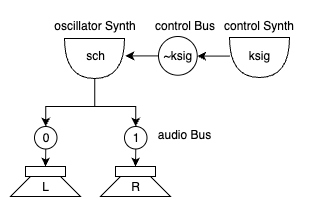
\includegraphics[scale=0.7]{../img/kbus.png}
\end{center}

Let's define a SynthDef that generate different types of control signals and a control Bus:
\begin{itemize}
\tightlist
\item 0 $\rightarrow$ MouseX position.
\item 1 $\rightarrow$ MouseY position.
\item 2 $\rightarrow$ random values at a determined frequency.
\end{itemize}

For each we can set the range (min, max).

\begin{lstlisting}[frame=single, caption=Control signals model,label=control] 
SynthDef(\ksig,{arg type=0, range=#[0,1], freq=1, busOut=0;
                var sig;
	                sig = Select.kr(type,
                                [MouseX.kr(range[0], range[1]),
                                 MouseY.kr(range[0], range[1]),
                                 LFNoise1.kr(freq).range(range[0], range[1])
                                ]);
	            Out.kr(busOut,sig)
        }).add;

x = Bus.control(s, 1);   // a control bus (server, n_canali)
\end{lstlisting}

The SynthDef

\begin{lstlisting}[frame=single, caption=Scratcher model] 
SynthDef(\sch, {arg buf=0, smooth=0.02, amp=0, pos=0, pan=0;
                var pnt, sig;
                    pnt = Lag.kr(pos.linlin(0,1,0,BufFrames.kr(buf)),smooth);
                    sig = BufRd.ar(1, buf, K2A.ar(pnt));
                    sig = Pan2.ar(sig * amp, pan);
                Out.ar(0, sig)
        }).add;
\end{lstlisting}

The Synths.

\begin{lstlisting}[frame=single] 
Buffer.freeAll;
b = Buffer.read(s,"/absolute/path/to/file.wav");

k = Synth(\ksig, [\type,0, \range, [0, 1], \busOut, x]);   // Synth per ksig
a = Synth(\sch, [\buf,b, \amp,1, \pos, x.asMap, \smooth,0.02, \pan,0]);
\end{lstlisting}

Change the smoothing time.

\begin{lstlisting}[frame=single] 
a.set(\smooth,0.2);
\end{lstlisting}

Apply a random control signal and change its sub audio freuency.

\begin{lstlisting}[frame=single] 
p.set(\type, 2, \freq, 2);
\end{lstlisting}

\subsection{Structures, DAW and scoring}\label{structures-daw-and-scoring}

In the previous paragraph we saw some tools for generating the sound palette with which to create the composition.

Now we need to string them together into a formal structure.

Two options:

\begin{itemize}
\tightlist
\item record the musical objects into soundfiles and edit them in a DAW.

\begin{enumerate}
\def\labelenumi{\arabic{enumi}.}
\tightlist

\item create the soundfile.
\begin{lstlisting}[frame=single] 
s.prepareForRecord("/absolute/path/to/prova.wav", 2); // path, channels
\end{lstlisting}

\item start recording and sound.
\begin{lstlisting}[frame=single] 
s.record;
a = Synth(\ksig, [\buf,b, \amp,1, \pan,0, \freq, 3, \gate, 1])
\end{lstlisting}

\item fade out and stop recording.
\begin{lstlisting}[frame=single, caption=Recording sound] 
r = Routine({
            a.set(\fOut, 2, \gate,0); // Trig fade out
            3.wait;                   // Wait for fadeout end
            s.stopRecording;          // Stop recording
            }).play
\end{lstlisting}
\end{enumerate}

You can now open it in a DAW and mix with others in a structure.


\item compose the entire structure directly in SuperCollider (scoring).

\begin{enumerate}
\def\labelenumi{\arabic{enumi}.}
\tightlist

\item define all the SynthDefs.
\begin{lstlisting}[frame=single] 
SynthDef(\grain, {arg buf=0, pos=0, dur=0.2, amp=0, trsp=0, dir=1, pan=0,
	                  t_gate=0, atk=0.1, done=2;
                  var sig,env;
                      sig = PlayBuf.ar(1, buf,
                            BufRateScale.kr(buf) * trsp.midiratio * dir,
                            t_gate,
                            BufSampleRate.kr(buf)* pos );
                      env = Env.perc(atk, dur-atk);
                      env = EnvGen.kr(env,t_gate,doneAction:done);
                      sig = Pan2.ar(sig * env * amp, pan);
                Out.ar(0,sig)
                }).add;
SynthDef(\ksig,{arg buf=0, amp=0,frq=0.1,fIn=0.2,fOut=0.2,pan=0,
                    gate=0,done=2;
                var punta,sig,fade;
                    punta = LFCub.ar(frq).range(0,BufFrames.kr(buf));   
                    sig   = BufRd.ar(1, buf, K2A.ar(punta));
                    fade  = Linen.kr(gate,fIn,1,fOut,done);
                    sig   = Pan2.ar(sig*amp.lag(0.2)*fade,pan);
                Out.ar(0, sig);
        }).add;
\end{lstlisting}

\item define the different sound objects within Routines or Synths or functions.
\begin{lstlisting}[frame=single] 
Buffer.freeAll;
b = Buffer.read(s, "/absolute/path/to/file.wav");

~durs = [0.9,0.8,0.7,0.6,0.5,0.4,0.3,0.2,0.1];       
~pos  = [0.1,0.3,0.5,0.7,0.9,1.1,1.3,1.5,1.7];
~atk  = [0.01,0.02,0.43,0.04,0.35,0.06,0.57,0.08,0.89];    
~pan  = 1;  
~obj1 = Routine({
                inf.do({arg id;                              
                        Synth(\grain, [\buf, b, 
                                       \amp, 0.4, 
                                       \pos, ~pos.foldAt(id), 
                                       \done, 2, 
                                       \atk, ~atk.foldAt(id), 
                                       \t_gate, 1]);
		                    ~durs.foldAt(id).wait;                 
                        });
                });

~amps = [0.01, 0.4, 0.1, 0.6];
~pos  = [0.5, 1.4, 3.1, 2.6, 0.5, 2.8];
~obj2 = Routine({
                inf.do({arg id;             
                        ~pan = ~pan * -1;        // flip flop                 
                        Synth(\grain, [\buf, b, 
                                       \amp, ~amps.foldAt(id),
                                       \dur, 0.2, 
                                       \pos, ~amps.wrapAt(id),
                                       \done, 2, 
                                       \atk, 0.01, 
                                       \pan, ~pan,
                                       \t_gate, 1]);
		        0.3.wait;                 
                       });
                });
\end{lstlisting}

\item arrange it in a score (we can specify the temporal events or bars as comments).
\begin{lstlisting}[frame=single] 
~score = Routine({
                  2.do({                    // Ritornello (loop)
                        ~obj2.reset.play(t);         // 0 Start obj2
                        3.wait;
                        3.do({                       // 3 Ritornello 
                              ~obj1.reset.play(t);   // Start obj1
                              4.wait;
                              ~obj1.stop;            // Stop obj1
                              1.wait});
                        ~obj3 = Synth(\ksig,[\buf,b, // 18 Start obj3
                                             \amp,0.1,
                                             \fIn,3,
                                             \frq,2,
                                             \gate,1]); 
                        2.wait;
                        ~obj2.stop;                // 20 Stop obj1
                        1.wait;
                        ~obj1.reset.play(t);       // 21 Start obj2
                        ~obj3.set(\fOut, 4, \gate, 0); // Fout obj3
                        3.wait;
                        ~obj1.stop;                // Stop obj1
                        1.wait;                    // 25 End obj2                                        
                        })
                })
\end{lstlisting}

\item play the score.
\begin{lstlisting}[frame=single, caption=Scoring] 
~bpm = 100;                         
t    = TempoClock.new(~bpm/60); // Set bpm tempo

~score.reset.play(t);
\end{lstlisting}
\end{enumerate}
\end{itemize}

Through this modular procedure, we can define the structure of: 
    
\begin{enumerate}
\tightlist
\item the entire piece. 
\item individual tracks. 
\item sections and fragments.
\end{enumerate} 

We can represent it in a graphic score.

\begin{center}
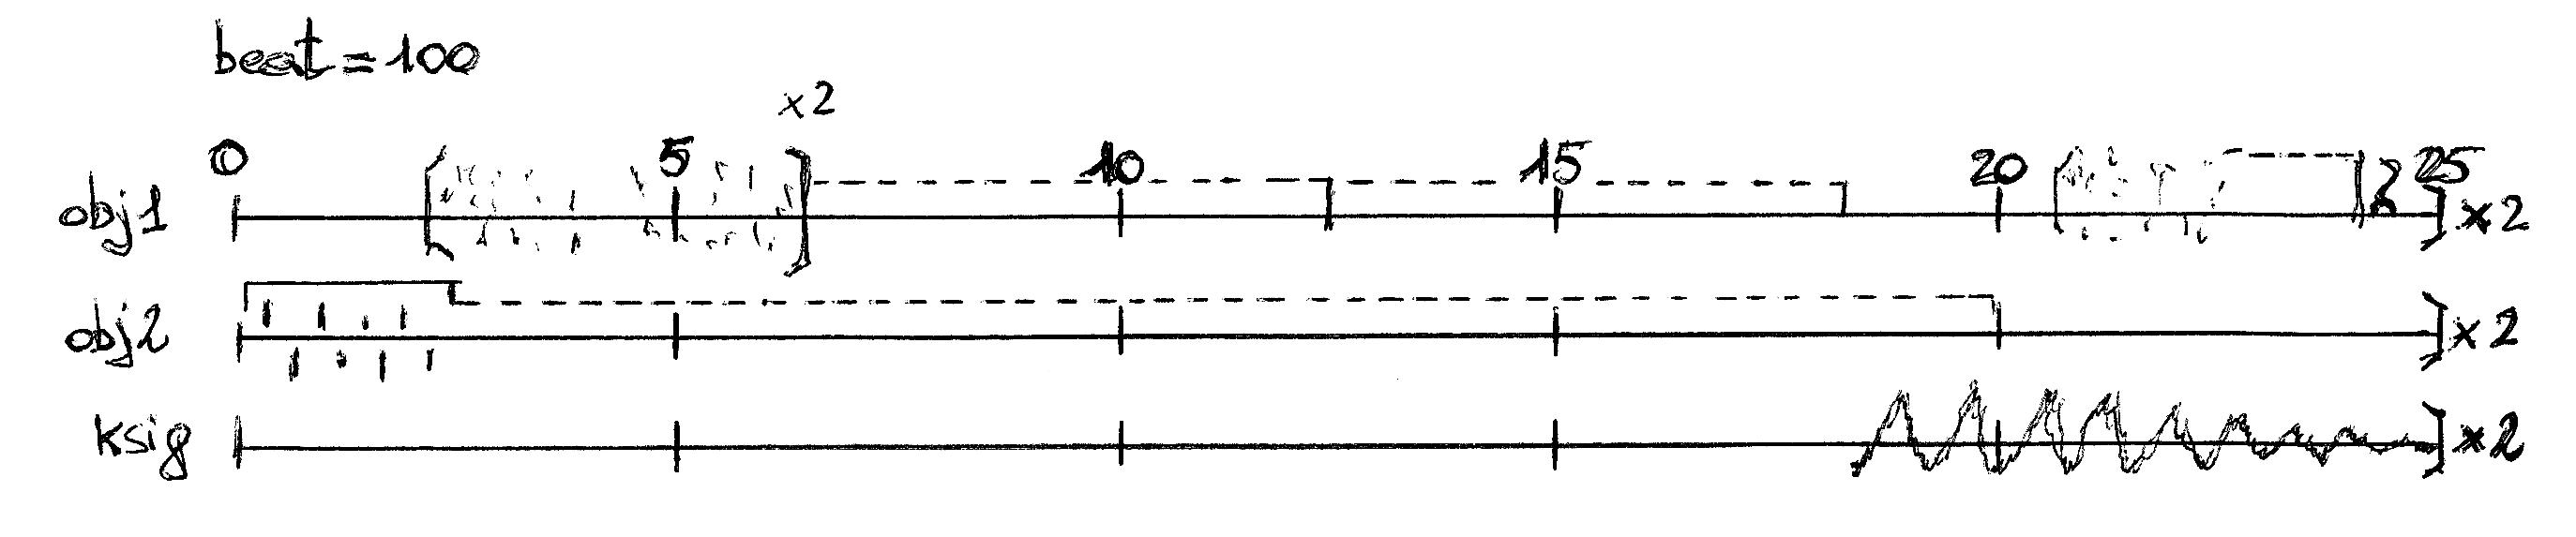
\includegraphics[scale=1]{../img/scores.png}
\end{center}

Link to an example of a graphic score of a historical piece by J.C.Risset - \href{http://www.musicaecodice.it/gitmedia/emc/3_media/risset1.mp4}{Sud} (1984-85).

\subsection{Composition sketches proposal}\label{composition-sketches-proposal}


\textbf{Sound palette}

\begin{enumerate}
\def\labelenumi{\arabic{enumi}.}
\tightlist
\item design and create a sound palette starting from a short soundfile (2-10 seconds).
\item group the different sets of musical objects made by morphological characteristics.
\end{enumerate}

\textbf{Fixed media work or sound design}

Two different strategies:

\begin{itemize}

\item bottom to top.

   \begin{enumerate}
   \def\labelenumi{\arabic{enumi}.}
   \tightlist
   \item choose one to three short sound texts (soundfiles). 
   \item analyze the morphological structure of the sound files (microform) 
   \item starting from a musical object begin to compose the general structure (macroform) step by step in a DAW or through scoring techniques. At each step creating new musical objects and their development into microstructures. Idea of the macroform will not be clear until the end of the process.
  \end{enumerate}
    Macroform develops from microstructure.

\item Top to bottom.

  \begin{enumerate}
  \def\labelenumi{\arabic{enumi}.}
  \tightlist
  \item define a global formal structure in a graphical sketch.
  \item design and create a sound palette based on the types of sounds described in the sketch according to the principles set out in the chapter (rules or \textit{libero arbitrio}).
  \item realize the sketch in a DAW or through scoring techniques.
  \end{enumerate}

  Microstructures fill the macroform.
\end{itemize}